\documentclass[12pt]{article}

% Packages
\usepackage{amsmath}
\usepackage{graphicx}
\usepackage{booktabs}
\usepackage{natbib}
\usepackage{hyperref}
\usepackage{geometry}
\usepackage{mathptmx} % Times font
\usepackage{multirow}
\usepackage{array}
\usepackage{placeins}

% Page setup
\geometry{margin=1in}

% Hyperref setup
\hypersetup{
  colorlinks=true,
  linkcolor=blue,
  citecolor=blue,
  urlcolor=blue
}

\title{\new{Processing Cost Tracks Representational Trajectory Beyond the Predictive Distribution, in Comprehension and Production}}

\author{Elan Barenholtz\\
Machine Perception \& Cognitive Robotics Laboratory\\
Department of Psychology / Center for Complex Systems\\
Florida Atlantic University\\
\texttt{elan.barenholtz@fau.edu}}

\date{}

% ---- REVIEW AID: new/changed text in v2 is wrapped in \new{...} and set bold.
% ---- To turn the highlighting off, change the definition to \newcommand{\new}[1]{#1}
\newcommand{\new}[1]{#1}   % highlighting off for submission (set to {\bfseries #1} to mark v2 changes)

\begin{document}

\maketitle

\begin{abstract}
\new{Surprisal theory holds that the cost of processing a word is a function of its probability under the current predictive distribution: the history is used to compute the distribution and then discarded. We test that sufficiency claim on both sides of the channel. We define trajectory extrapolation error---the distance between a word's hidden state in a transformer language model and a linear extrapolation from the preceding three states---and report four results. First, the measure predicts self-paced reading time beyond surprisal in the Natural Stories corpus ($\Delta\text{AIC} = 78$; 67\% of 171 participants positive), survives a control built from four surprisal estimates spanning GPT-2 and Pythia, partially replicates in a second self-paced corpus of 2,000 participants (61\% sign agreement against a pre-specified 65\% criterion), and, in a preregistered test, does not reduce to constituent structure: the effect is strongest precisely where no constituent closes (80\% of participants within phrases), the reverse of syntactic wrap-up. Second, the effect is not carried by the shape of the predictive distribution. Extrapolation error is nearly orthogonal to entropy, confidence, and concentration ($|r| \le .07$), and the reading-time effect survives---indeed strengthens---with all four distribution functionals in the model and within cells matched on the distribution (75\% of participants, $p = 8 \times 10^{-14}$). Third, production shows the same cost at the same grain: in the time-aligned Buckeye corpus, speakers pause longer before words with high extrapolation error, controlling for surprisal and the distribution functionals (68\% of 40 speakers, $p = .003$; a preregistered pass on a 7-speaker subset replicated exactly on the 33 unseen speakers), with a directionally consistent partial replication across 4,747 Switchboard conversation sides ($p = 5 \times 10^{-73}$; 61\% against the 65\% criterion) and no effect at intonation-unit launches, where planning dominates. Fourth, the corresponding structure in text is fully absorbed by a stronger model's distribution: in a preregistered rank test with an AI-sampled negative control, human continuations are distinguishable from GPT-2 Small's samples but indistinguishable from GPT-2 XL's. The current predictive distribution is sufficient for what people write, and insufficient for what it costs them to read or to speak: the trajectory dependency lives in the processor, not the text.}

\end{abstract}

\newpage

\section{Introduction}

Human language comprehension unfolds sequentially. Words arrive one at a time, and the reader or listener must build an interpretation incrementally, each word updating and extending the representation constructed from those that came before. Understanding this incremental process is a central problem in psycholinguistics, and the word-by-word variation in reading times has long served as its primary empirical signature. A core regularity in this signature is that words predictable in context are processed more quickly than words that are not. The dominant computational framework for explaining this regularity is surprisal theory \citep{hale2001,levy2008}, which holds that the cost of processing a word is proportional to its negative log probability given the preceding context. % [v2] DELETED: the v1 sentence beginning "The framework follows naturally from
% information-theoretic considerations..." committed to a belief-updating
% mechanism (comprehender maintains a probability distribution; low-probability
% words impose an update cost). Removed rather than rewritten.
Surprisal has been remarkably successful as a predictor of reading times across self-paced reading \citep{smith2013}, eye-tracking \citep{demberg2008}, and neural measures \citep{frank2015}.

Computing surprisal requires an underlying predictive model. Early work used n-gram models and probabilistic grammars \citep{hale2001,demberg2008,roark2009}, which provided useful but limited estimates of word predictability. Transformer-based language models have since become the standard tool \citep{goodkind2018,wilcox2020,schrimpf2021}, largely because their surprisal estimates are better predictors of human reading times than those from earlier models, and because they can condition on arbitrarily long contexts rather than fixed windows. They are also a natural fit because they are themselves sequential processors: trained to predict the next token given the preceding sequence, they build rich internal representations that update incrementally as each word is encountered. Because these models are trained on human-produced text, the statistical structure they capture --- sensitivity to context, coherence, discourse --- is the same structure latent in that production, which is what makes their surprisal a useful index of the predictive regularities to which human comprehenders are sensitive.

\new{Surprisal is computed from the entire preceding context, so it is not a memoryless quantity in the way an n-gram statistic would be. Its commitment lies elsewhere. Surprisal reduces the context to a distribution over the next word, and then to a single number drawn from that distribution, and surprisal theory treats that number as sufficient: given how unexpected a word was, nothing further about how the interpretation reached its current state should bear on the cost of processing it. The history is used to compute the statistic and then discarded. This is a substantive assumption rather than a technical convenience, and it is testable.}

\new{There are two distinct ways the data could exceed that scalar, and they have very different theoretical consequences. The first is that the cost function uses more of the current distribution than its value at the observed word: its entropy, its concentration, the probability mass on competitors. A comprehender of that kind is still a current-state processor; surprisal theory would need a richer functional, not a different architecture. The second is that cost depends on how the state was reached---on the recent path of the interpretation through its representational space, over and above anything the current distribution encodes. A dynamical tradition has long treated comprehension in exactly these terms, as a process evolving through a continuous state space \citep{tabor1999,spivey2007,cho2017}, and only this second possibility is a genuine departure from the sufficiency assumption. Distinguishing the two requires measuring the trajectory and the distribution separately, and testing each against processing cost with the other controlled. That is what this paper does.}

\new{The same sufficiency question has a production side, and the two sides constrain each other. Language production is sequential and locally planned: speakers plan a few words ahead, execute, and re-plan \citep{levelt1989,ferreira2002}. If the processing system that generates speech is sensitive to representational trajectory, that sensitivity should surface in production \emph{timing}---hesitation before words that depart from the recent path---even if it leaves no measurable residue in the produced text itself. The distinction matters: any lawful trajectory structure in what people produce is a statistical regularity of text, and a sufficiently good conditional model will absorb it into its predictive distribution. Content, in other words, cannot ultimately separate a trajectory mechanism from statistics; timing can. We therefore test the timing of production directly, and we test the content claim as well, with a design built to fail if the structure is absorbable.}

Testing whether trajectory dynamics shape human processing requires a way to measure trajectory structure in an evolving interpretive representation. Modern transformer language models like GPT-2 \citep{radford2019} provide one. Their hidden states encode a rich, incrementally updated representation of the context processed so far, and because the model is trained on human-produced text, these representations come to reflect not only the predictive structure that surprisal captures, but also other latent regularities of production --- including the short-horizon continuity of how each word's representation extends from those of its predecessors. Here, we introduce a simple measure that we call trajectory extrapolation error. At each word position, we fit a linear trajectory to the hidden states of the preceding $k$ words (typically $k = 3$), extrapolate one step forward, and measure the Euclidean distance between this predicted position and the actual hidden state. The measure captures the degree to which the current word deviates from where the representation was heading: high extrapolation error means the representation was moving in one direction and the current word forced it somewhere else; low error means the current word continued the established drift.

The logic of comparing trajectory extrapolation error against surprisal is asymmetric. Surprisal is expected to predict processing cost under either tradition, since improbable words tend to disrupt trajectories; finding that surprisal matters does not distinguish between the frameworks. Finding that trajectory extrapolation error adds independent explanatory power beyond surprisal would, by contrast, be informative: it would suggest that the dynamical character of comprehension contributes to processing cost in a way that word-level prediction error does not capture. Two words with identical conditional probability receive identical surprisal even if one continues an established interpretive trajectory and the other forces a sharp representational turn, and any cost difference between such words is evidence for directional dynamics in comprehension. This asymmetry is not a limitation of the language models from which surprisal is derived: their hidden states already carry the trajectory information, but surprisal as an output measure collapses it to a scalar.

\new{This paper is concerned with whether the dynamics that surprisal discards are psychologically relevant.} Human processing unfolds under strong constraints of recency and local influence \citep{gibson1998,lewis2005}, meaning that recent words dominate the current interpretive state. Under such constraints, the trajectory of the interpretation over the last few words is the comprehender's best available signal about where things are heading. Sensitivity to this trajectory, tracking the recent drift of the interpretation rather than treating each word as an independent event, would constitute an efficient processing strategy that exploits the local momentum of natural language. Garden-path sentences provide an intuitive illustration: in ``The horse raced past the barn fell,'' each word after ``raced'' reinforces the main-verb interpretation, building momentum in one direction, and the cost at ``fell'' reflects not just the word's unexpectedness but the reversal of accumulated interpretive direction. But if trajectory sensitivity is a general feature of human processing, the phenomenon should not be limited to garden paths. Any word that forces the interpretation off its recent trajectory should incur a cost, even in ordinary text, and this cost should be measurable independently of surprisal.


\new{Our primary dataset is the Natural Stories corpus \citep{futrell2018}, where the measure can be evaluated over thousands of word positions of naturalistic connected text read by 181 participants. This is the larger and less constrained test, and it is where our analytic decisions---the model specification, the use of subject-level inference, and the criteria for judging an effect reliable---were made. We then turn to the Classic Garden Path materials of the SAP Benchmark \citep{huang2024}, carrying those decisions over. The control set is not identical across the two corpora: connected text and 13--17 word isolated sentences require position to be handled differently, and the sentence corpus uses distance from sentence start and end with quadratic terms in place of the running-text position and previous-reading-time controls. The inferential criteria, the measure, and the model form are unchanged. These materials were of interest for a specific reason: the disambiguating word of a garden-path sentence is a theoretically motivated locus of trajectory disruption, a point at which the interpretation is known to reverse, and if the measure indexes the cost of such reversals it should register there in particular. We ask two questions of them. The first concerns the ambiguity manipulation: does the difference in extrapolation error between a garden-path sentence and its unambiguous control predict the difference in reading time, across items? The second sets the manipulation aside and treats the materials as what they also are---a second self-paced reading corpus, 144 syntactically difficult sentences read by 2,000 participants---and asks whether the Natural Stories result holds there.}

\new{Both corpora use self-paced reading, which delivers words serially, one at a time and only on request. We take up the question of whether the effect extends to reading with free eye movements separately; the evidence reported here concerns serial presentation.}

\new{An immediate objection must be met before any of this can be interpreted: constituent structure. Words within a phrase are related, so their representations might move coherently for purely syntactic reasons, boundaries might supply the turns, and the reading-time effect might be syntactic wrap-up. We test this directly, in a preregistered analysis, by classifying every word transition by its position in the corpus's constituency parses (Section~\ref{sec:syntax}).} Three additional analyses clarify what the measure captures. A displacement control assesses whether the contribution of extrapolation error reduces to the magnitude of representational change at each word. A direction-preservation analysis on the Natural Stories corpus characterizes the temporal scale of the underlying trajectory structure in the model. Finally, \new{a cross-architecture replication using Pythia (which uses Rotary Position Embeddings rather than the absolute positional embeddings of GPT-2) tests whether any effect of trajectory structure generalizes across model scale and positional encoding scheme, and a series of surprisal controls drawn from larger models tests whether the effect is a residual of poor predictability estimation by any one model}.

\new{The reading-time results, however extensively controlled for surprisal, leave the first of the two possibilities above open: a cost function over richer functionals of the current distribution could mimic trajectory sensitivity if the trajectory measure happened to covary with distribution shape. Section~\ref{sec:distsuff} closes this, in a preregistered analysis: the measure is nearly orthogonal to entropy, confidence, and concentration, and the effect survives both covariate control and distribution matching. Section~\ref{sec:production} then takes the question to production, testing whether speakers' silent pauses before each word track the same measure in time-aligned spontaneous speech (Buckeye, Switchboard), with the same distribution functionals controlled. Section~\ref{sec:content} reports the content test: a preregistered rank analysis asking whether the words humans actually produce are distinguishable from samples drawn from a model's own predictive distribution, across a ladder of model strengths. Its outcome---distinguishable for a weak model, indistinguishable for a strong one---is what licenses the paper's framing: the trajectory dependency is a property of language \emph{processing}, not of language.}

\section{Method}

\subsection{Materials}

\paragraph{Garden-path sentences.} To test the trajectory effect at a controlled, theoretically motivated locus of disruption, we used the Classic Garden Path subset of the SAP Benchmark \citep{huang2024}, a large-scale syntactic ambiguity processing dataset. The subset contains 24 items covering three structural types: main-verb/reduced-relative (MVRR; e.g., ``The horse raced past the barn fell''), NP/S direct-object/sentential-complement (e.g., ``The suspect showed the file deserved more attention''), and NP/Z transitive/intransitive (e.g., ``While the man hunted the deer ran into the woods''). Each item appeared in ambiguous and unambiguous conditions, where the unambiguous version included an overt syntactic marker (e.g., a relative pronoun) that prevents the garden-path misparse. Human reading-time data were collected via self-paced word-by-word reading from over 2,000 participants. Reaction times were filtered to exclude responses below 100 ms or above 5,000 ms.\new{\footnote{An earlier version of this paper (arXiv:2606.05346v1) reported a reading-time analysis restricted to the critical region of these materials. That analysis contained a sample-construction error and is withdrawn; see the version note. The materials are analysed here in two ways: as an ambiguity manipulation at the item level, and as a corpus of connected text.}} \new{These sentences were presented in isolation rather than embedded in running text, so fit windows near the start of a sentence could in principle include the first token, whose hidden-state magnitude is anomalously large in transformer models \citep{xiao2023}. We therefore begin every fit window at the second token, which excludes that position by construction and restricts the analysis to word positions 5 and later.}

\paragraph{Natural Stories.} To evaluate the same measure across thousands of word positions in naturalistic text, we used the Natural Stories corpus \citep{futrell2018}, which consists of 10 naturalistic narratives totaling approximately 10,000 words. Self-paced reading times were collected from 181 participants, yielding \new{848,875} observations after filtering to 100--3,000 ms\new{; 813,621 remain after merging to the measure sample, and 812,730 from 178 participants enter the fitted models once the previous-word control is defined}. We processed each story through GPT-2 in overlapping chunks to accommodate the model's 1,024-token context limit, computing hidden states and surprisal at every word position.

\subsection{Trajectory Extrapolation Error}

\paragraph{Definition.} Let $h_t$ denote the hidden-state vector at word position $t$ in a given layer of a transformer language model. For a window of size $k$, we fit a linear trajectory to the hidden states at positions $t{-}k$ through $t{-}1$ by ordinary least squares. The extrapolated position at the next time step is the linear prediction at time $k$, and trajectory extrapolation error is defined as the Euclidean distance between the extrapolated and actual hidden states (see Figure~\ref{fig:schematic} for a schematic illustration). This quantity measures how far the representation landed from where it was heading, given the trajectory established by the preceding $k$ words.

\begin{figure}[!ht]
\centering
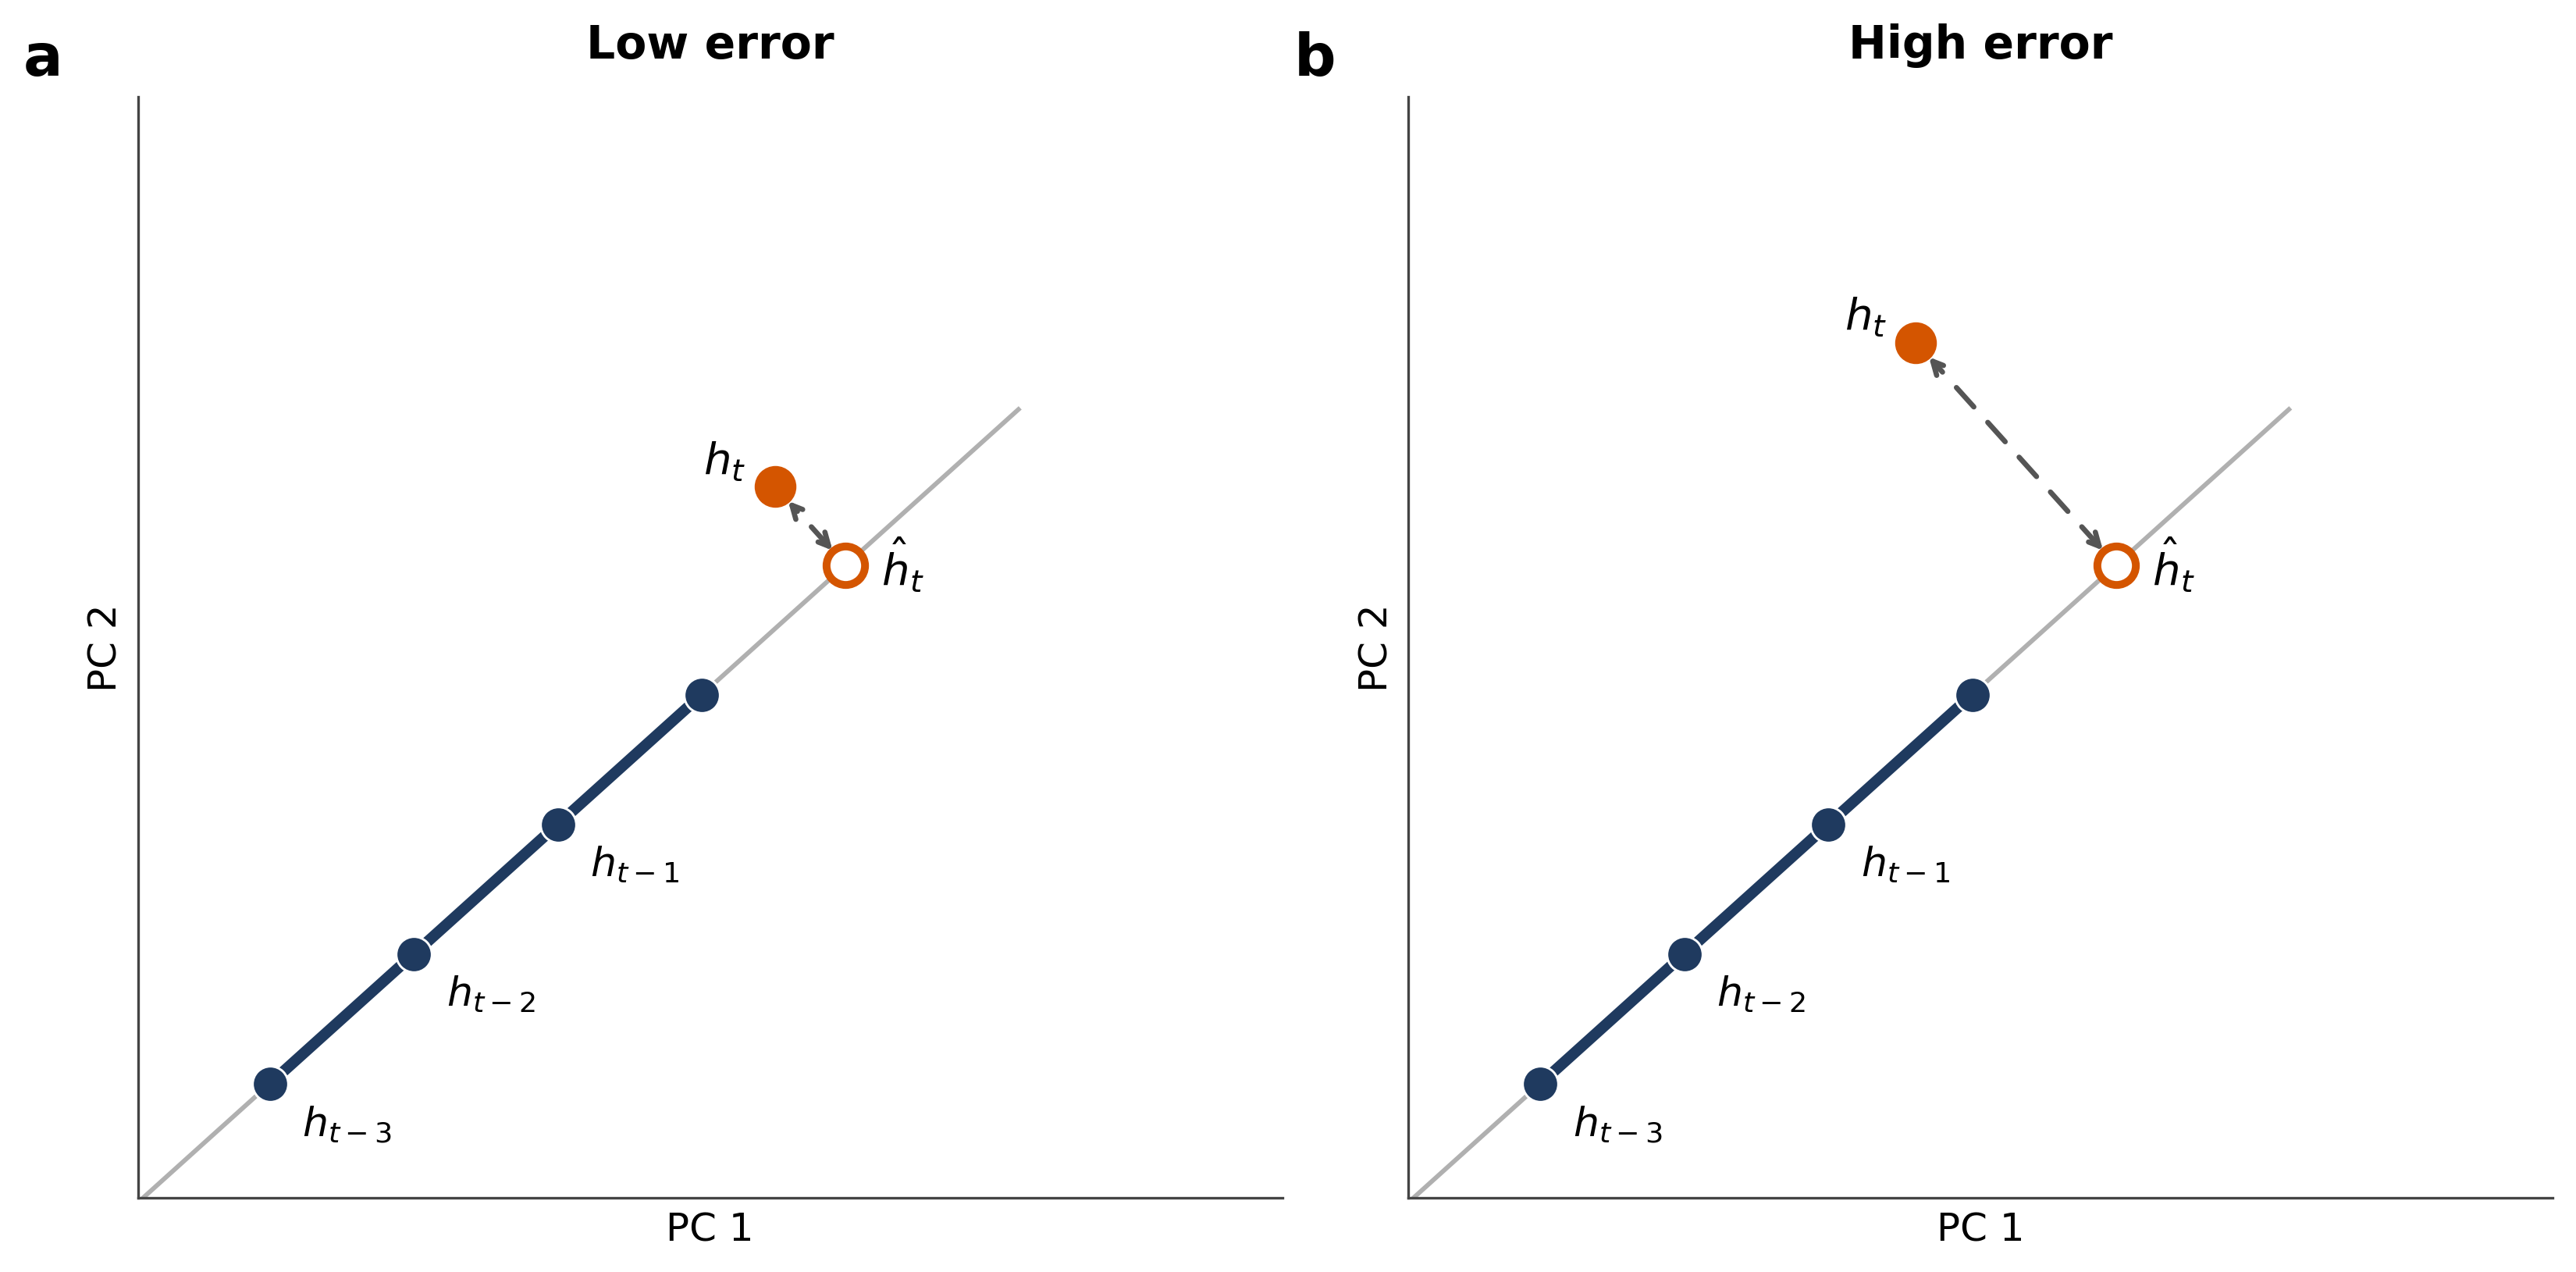
\includegraphics[width=\textwidth]{fig1_schematic.png}
\caption{Schematic illustration of trajectory extrapolation error. Each point $h_t$ represents the model's hidden-state vector at word position $t$, projected into a two-dimensional principal-component space for visualization. A linear trajectory is fit to the hidden states at the preceding $k$ positions (here $k = 3$: $h_{t-3}$ through $h_{t-1}$) and extrapolated one step forward to produce a predicted position (open circle, $\hat{h}_t$). Trajectory extrapolation error is the Euclidean distance between this predicted position and the actual hidden state $h_t$ (filled orange circle). (a) Low error: the current word's hidden state falls near the extrapolated position, continuing the established trajectory. (b) High error: the current word (e.g., a garden-path disambiguator) forces the hidden state far from the extrapolated position.}
\label{fig:schematic}
\end{figure}

\paragraph{Parameter selection.} We computed extrapolation error using GPT-2 (117M parameters; \citealp{radford2019}), which sits near the sweet spot for reading-time prediction identified by \citet{oh2023a}. We tested two layers: layer 6 (an intermediate layer) and the final layer (layer 12). We focus primarily on layer 6 because intermediate layers are known to capture syntactic representations more effectively than output layers in transformer models \citep{hewitt2019,jawahar2019}. \new{The 3-word window and layer 6 were fixed in the previous version of this work and are retained here unchanged. We report the window sweep on the corrected pipeline for transparency, because it does not favour that choice: entered in the headline specification, $k = 2$ improves fit by $\Delta\text{AIC} = 539.6$ ($\beta = +0.0072$, 84.2\% of participants positive) and $k = 7$ by $85.5$, against $78.4$ for the reported $k = 3$. Fit degrades from $k = 15$ and reverses sign by $k = 30$. We do not adopt the best-fitting window, because selecting the parameter on the outcome variable is precisely the researcher degree of freedom this paper is otherwise at pains to avoid; $k = 3$ is retained for continuity with the earlier report. A reader should treat the window as a fixed prior choice rather than an optimised one, and note that the measure at $k = 2$---the discrete second difference of the hidden-state sequence---is a different quantity that merits separate investigation. Layer and polynomial-degree variants are not present in the locked sample and were not re-verified under the corrected pipeline.} For sentences with subword tokenization, we used the hidden state at the last subword token of each word.

\subsection{Direction Preservation Analysis}

To characterize the trajectory structure underlying extrapolation error, we computed a direction preservation measure on the Natural Stories corpus. At each word position, we measured the absolute cosine similarity between the fitted trajectory direction (from the preceding $k$ words) and the actual displacement vector at the current word and at 1, 2, and 3 steps ahead. This measures whether the direction of representational change at one position predicts the direction of change at subsequent positions. For random vectors in 768-dimensional space, the expected absolute cosine similarity is approximately 0.029, providing a chance baseline.

\subsection{Statistical Analyses}

We fit linear mixed-effects models predicting log-transformed reading times, with random intercepts for participants. All continuous predictors were $z$-scored prior to entry. \new{Word frequency is the Zipf value of the lowercased word with attached punctuation removed. We note this explicitly because the frequency values used in v1 were derived without that normalisation and were zero for 19.7\% of tokens, including ordinary words carrying attached punctuation and words differing only in case; all frequency-dependent analyses reported here have been recomputed.} The baseline model (M0) included word length, word position, previous log RT, and log word frequency (Zipf score; standard psycholinguistic control, e.g., \citealp{smith2013}) as lexical controls. We then tested a series of nested models: M1 added surprisal; M2 added trajectory extrapolation error. Model comparisons were evaluated using the Akaike Information Criterion (AIC), the Bayesian Information Criterion (BIC), and likelihood ratio tests. AIC estimates out-of-sample prediction error, with lower values indicating better fit; BIC applies a stronger penalty for model complexity and is more conservative. For the Natural Stories analysis, we additionally included log word frequency as a control and tested the independence of surprisal and extrapolation error via correlation and a tercile-based dissociation analysis. As a further control, we tested whether extrapolation error reduces to simple one-step representational change by comparing it with embedding displacement ($\|h_t - h_{t-1}\|$) in a joint model including both measures alongside surprisal and lexical controls.

\new{Because a pooled model over hundreds of thousands of observations can register an effect that no individual reader shows, the headline reading-time analyses in both corpora were additionally estimated separately within each participant and tested across participants. We treat an effect as reliable when the group-level test reaches $p < .01$ and at least 65\% of participants share the sign of the coefficient. These criteria were fixed on Natural Stories and applied unchanged thereafter. Where sign agreement is reported, it is accompanied by a permutation floor obtained by shuffling the measure within participant and refitting.}

\new{To test the robustness of the effect across model scale and architecture, we repeated the Natural Stories analysis using Pythia-160M and Pythia-410M \citep{biderman2023}, which use Rotary Position Embeddings rather than the learned absolute position embeddings of GPT-2, testing the proportionally equivalent mid-layer of each. All models were evaluated on identical rows and identical participants.}

\new{Two comparisons were run on the garden-path materials. The first treats them as an ambiguity manipulation: for each item we computed the ambiguous-minus-unambiguous difference in extrapolation error, in surprisal, and in mean log reading time at the disambiguating word, and asked whether the model-derived differences predict the behavioural one across items, with and without fixed effects for construction. The second sets the manipulation aside and treats the materials as a reading-time corpus, using the same specification developed on Natural Stories.}

\new{\subsection{Distribution Functionals}

To test whether any trajectory effect reduces to the shape of the current predictive distribution, we computed four functionals of the model's next-word distribution at each position, from the logits in force at the word's first subword under the same chunked-context convention: Shannon entropy; collision (R\'enyi-2) entropy, an index of concentration; the log probability of the most probable token (confidence); and the log summed probability of the ten most probable tokens. These enter the reading-time analyses in two preregistered forms (criteria fixed in advance; preregistration in the repository): as covariates added to the headline specification, and as a matching variable, comparing words within cells defined by the joint quintiles of surprisal, entropy, and confidence, so that distribution shape is (coarsely) held fixed while the trajectory measure varies.

\subsection{Speech Corpora and Production Latency}

The production analyses use time-aligned spontaneous speech. The primary corpus is Buckeye \citep{pitt2007}, 286,707 analysed words of interview speech from 40 talkers with word-level alignments in which silent pauses appear as explicit timed intervals. The confirmation corpus is Switchboard-1 \citep{godfrey1992} with the ISIP manually corrected word alignments: 2,435 telephone conversations, 3.1 million words, silences again explicit. Two further corpora---the Santa Barbara Corpus \citep{dubois2000} and AMI \citep{carletta2007}---time speech only at the intonation-unit or segment level (their word-level times tile, absorbing pauses into words or units), and therefore support only unit-launch analyses, reported as boundary conditions.

The unit of analysis is the transition between consecutive words by the same speaker with only silence intervening; transitions containing interviewer speech, another speaker's onset, noise, or laughter are excluded (the pause must be a floor-holding silence). The dependent variable is $\log(1 + \text{pause duration in ms})$, clipped at 5 s. The predictor is the extrapolation error of the upcoming word, computed with the paper's standard conventions over the speaker's (Buckeye) or the interleaved conversation's (Switchboard) word sequence. Controls comprise the surprisal of the upcoming word, all four distribution functionals, Zipf frequency, word length, position within the fluent run, and cumulative position; all variables are demeaned within speaker to remove idiosyncratic pause style. Models are estimated within cluster (talker in Buckeye; conversation side in Switchboard) and tested across clusters with the standing criterion: group Wilcoxon $p < .01$ and at least 65\% of clusters sharing the positive sign. Designs, exclusions, and criteria were preregistered, with amendments documented before each corpus's dependent variable was related to the measure; the full audit trail is in the repository.}

\section{Results}

\new{Figure~\ref{fig:contrib} summarises the central result in advance of the
detail. In both self-paced corpora, trajectory extrapolation error accounts for
reading-time variance that surprisal and lexical frequency do not, at roughly a
third the magnitude of surprisal in Natural Stories and comparably to it in the
garden-path corpus. The evidence is stronger in Natural Stories, which meets our
pre-specified reliability criterion; the garden-path corpus does not, and is
reported as a partial replication. The sections below establish that result on the Natural
Stories corpus, carry the same measure, inferential procedure and reliability
criterion over to the garden-path materials with corpus-appropriate nuisance
controls, and
then examine what the measure is and is not capturing.}

\subsection{Natural Stories}

\new{\paragraph{Reading-time prediction.} Trajectory extrapolation error predicts self-paced reading time beyond surprisal and lexical controls ($\Delta\text{AIC} = 78.4$, $\beta = +0.0030$, $p = 3.1 \times 10^{-19}$, $N = 812{,}730$, 178 participants). For scale, in the same model $\beta(\text{surprisal}) = +0.0103$, $\beta(\text{word length}) = +0.0134$ and $\beta(\text{log frequency}) = +0.0045$: the trajectory effect is a little under a third the magnitude of surprisal, and is a second-order effect on reading time rather than a competitor to it (Figure~\ref{fig:contrib}).}

\new{\paragraph{Subject-level inference.} Because a pooled model over 812,730 observations can register an effect that no individual reader exhibits, we estimated the model separately within each participant. Of 171 participants with sufficient data, 115 (67.3\%) showed a positive coefficient (sign test $p = 7.6 \times 10^{-6}$; Wilcoxon $p = 2.4 \times 10^{-9}$; $t(170) = 6.74$). Thirty-two participants reached individual significance. We adopt this form of inference throughout, and take 65\% sign agreement together with a group-level $p < .01$ as the criterion for a reliable effect.}

\new{\begin{figure}[!htbp]
\centering
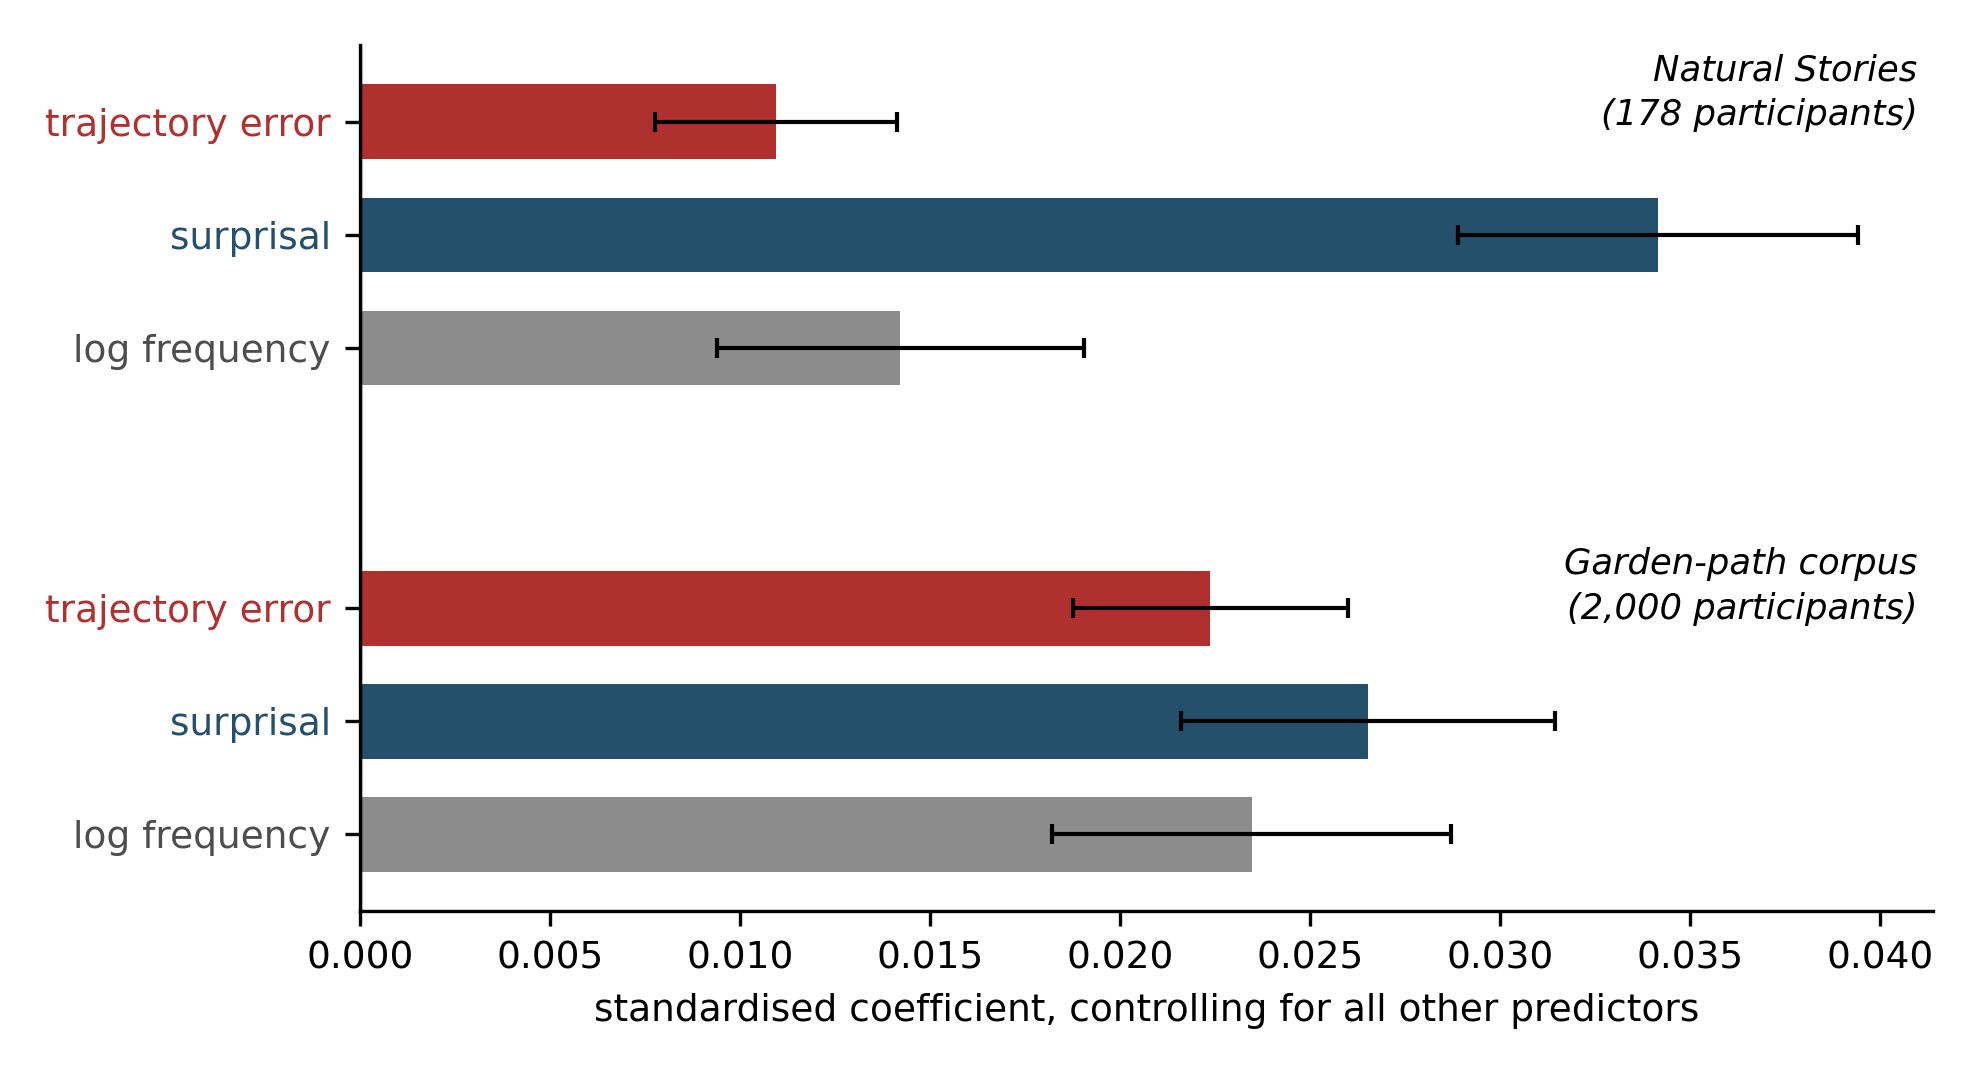
\includegraphics[width=0.72\textwidth]{fig_core.png}
\caption{Unique contribution of each predictor to self-paced reading time, in
both corpora. Each coefficient is estimated within participant with every other
predictor in the model, and averaged across participants; bars are 95\%
confidence intervals over participants. Trajectory extrapolation error accounts
for reading-time variance that surprisal and lexical frequency do not, at
roughly a third the size of surprisal in Natural Stories and comparably to it in
the garden-path corpus. Nuisance controls are included in every model but omitted from the plot; these
differ by corpus, being previous reading time and linear sentence position for
Natural Stories, and distance from sentence start and end with quadratic terms
for the garden-path corpus; word length is likewise omitted, being large enough in the garden-path
corpus ($+0.135$) to compress the remaining bars. Coefficients are standardised
within participant, so magnitudes are not directly comparable across corpora.}
\label{fig:contrib}
\end{figure}}

\new{\paragraph{Robustness.} The effect survives a control for word identity, centring the outcome and the remaining predictors within word type (2,919 types occurring five or more times; word length and frequency are constant within type and therefore drop out): it attenuates substantially but remains ($\Delta\text{AIC} = 23.1$, $p = 5.3 \times 10^{-7}$). A substantial share of the raw effect is therefore lexical, and a trajectory-specific component survives. Adding a punctuation covariate reduces it ($\Delta\text{AIC} = 70.0$), while restricting to punctuation-free words strengthens it ($\Delta\text{AIC} = 114.9$, $\beta = +0.0038$, $n = 716{,}641$).}

\paragraph{Independence of measures.} \new{Having established that the two measures contribute jointly, we turn to what distinguishes them.} The correlation between surprisal and extrapolation error at the word level was \new{$r = .31$, indicating that the two measures share roughly ten percent of their variance}. Whatever trajectory extrapolation error captures, it is not a nonlinear transformation of surprisal. \new{Because the measures are correlated, the evidence that each contributes independently rests on the analyses below rather than on the correlation.}

\paragraph{Dissociation analysis.} We split words into terciles on both surprisal and extrapolation error and examined mean log reading times in each cell of the resulting $3 \times 3$ matrix (Table~\ref{tab:dissociation}; Figure~\ref{fig:dissociation}). Words with high surprisal but low extrapolation error (surprising words that continue the trajectory) showed an increase of \new{$+0.029$} in log RT over the low/low baseline (\new{$t = 14.38$, $p = 8 \times 10^{-47}$}). Words with low surprisal but high extrapolation error (unsurprising words that disrupt the trajectory) showed an increase of \new{$+0.010$} (\new{$t = 5.43$, $p = 6 \times 10^{-8}$}). Both effects are significant, confirming that each measure captures unique variance in reading times.

\paragraph{Regression.} A mixed-effects model including both $z$-scored surprisal and $z$-scored extrapolation error confirmed independent\new{, additive contributions from each ($\beta_{\text{surprisal}} = +0.0102$, $\beta_{\text{extrapolation}} = +0.0030$). The additive model was preferred over one including their interaction ($\Delta\text{AIC} = 1.5$ in favour of the simpler model; interaction $\beta = +0.0002$, $p = .49$), indicating that surprisal and extrapolation error combine without amplifying or dampening each other. The margin is small, and we would not read the additivity as established, but there is no evidence of interaction.}

\begin{table}[!htbp]
\centering
\caption{Dissociation Matrix: Mean Log Reading Time by Surprisal $\times$ Extrapolation Error Tercile (Natural Stories)}
\label{tab:dissociation}
\begin{tabular}{lccc}
\toprule
 & \textbf{Low extrap error} & \textbf{Mid extrap error} & \textbf{High extrap error} \\
\midrule
\textbf{Low surprisal} & \new{baseline} & \new{+0.005} & \new{+0.010} \\
\textbf{Mid surprisal} & \new{+0.016} & \new{+0.016} & \new{+0.028} \\
\textbf{High surprisal} & \new{+0.029} & \new{+0.031} & \new{+0.041} \\
\bottomrule
\end{tabular}

\smallskip
\footnotesize
\textit{Note.} \new{Values are differences in mean log reading time from the low-surprisal / low-extrapolation baseline (5.717).} Off-diagonal cells represent the key dissociation: high surprisal / low extrapolation error reflects surprise without trajectory disruption; low surprisal / high extrapolation error reflects trajectory disruption without surprise. Both off-diagonal effects are independently significant (see text).
\end{table}

\begin{figure}[!htbp]
\centering
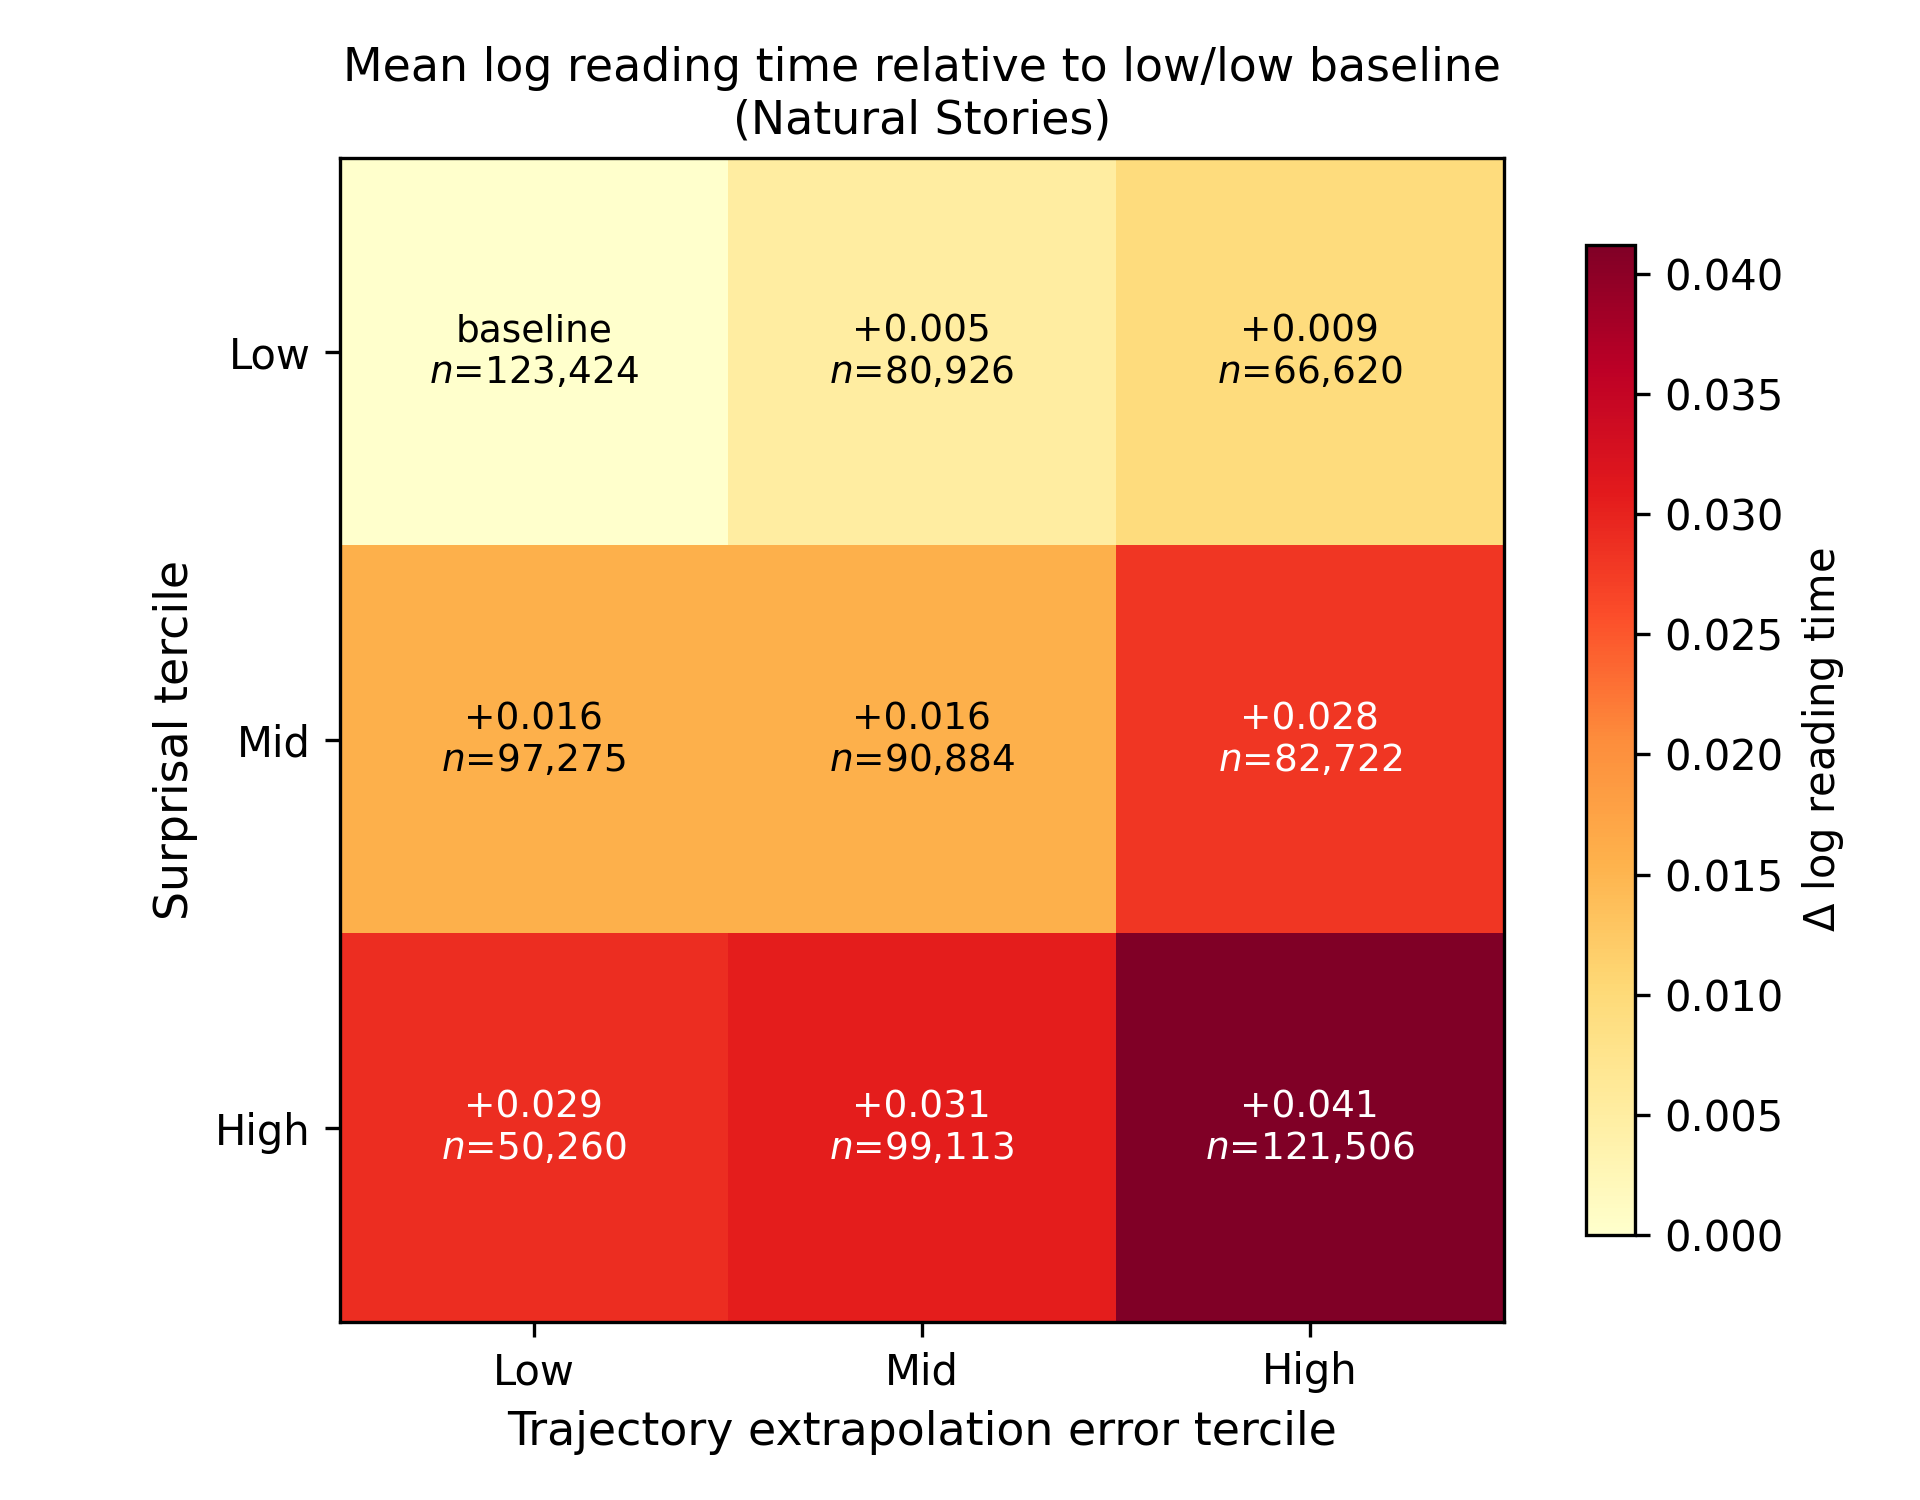
\includegraphics[width=0.8\textwidth]{fig3_dissociation.png}
\caption{Dissociation between surprisal and trajectory extrapolation error in Natural Stories. Heatmap shows mean log reading time in each cell of the $3 \times 3$ tercile matrix. The off-diagonal cells demonstrate that each measure captures unique variance: high surprisal / low extrapolation error (surprise without trajectory disruption) and low surprisal / high extrapolation error (trajectory disruption without surprise) both produce elevated reading times relative to the low/low baseline.}
\label{fig:dissociation}
\end{figure}

\FloatBarrier

\new{\subsection{Garden-Path Materials}

\paragraph{The ambiguity contrast.} Extrapolation error at the disambiguating word is higher in ambiguous than unambiguous sentences for NP/S ($+2.55$, 20 of 24 items) and NP/Z items ($+4.25$, 23 of 24), but reverses for main-verb/reduced-relative items ($-1.72$, 17 of 24, $t(23) = -3.26$, $p = .003$). Surprisal does not reverse for these items ($+5.23$, 23 of 24). The reversal reflects the item set rather than the measure. At the disambiguating word the three constructions produce nearly identical extrapolation error in the ambiguous condition (99.2, 98.3, 99.1), but the MV/RR unambiguous control sits at 101.0 against 95.7 and 94.8 for the other two. That control restores a full passive relative clause (``the horse \emph{that was} raced past the barn fell''), a low-frequency and structurally heavy construction that perturbs the trajectory about as much as the garden path does, so the difference score for these items compares two disrupted states rather than a disrupted state against a baseline. The disambiguating word and the three words entering its fit window are identical across conditions, so the difference is carried entirely by earlier context.

\paragraph{Item-level prediction.} Neither measure predicts the size of the human garden-path effect. Across 72 item $\times$ construction pairs, the ambiguous-minus-unambiguous difference in extrapolation error does not predict the corresponding difference in reading time once construction is controlled ($\beta = -0.019$, $p = .89$); surprisal does no better ($\beta = -0.035$, $p = .78$). This reproduces the central finding of \citet{huang2024} on their own materials.

\paragraph{Reading-time prediction across the corpus.} Setting the ambiguity manipulation aside, these 144 sentences constitute a self-paced reading corpus of syntactically difficult material read by 2,000 participants, and we analysed it as such: all words, all conditions, no region selection. Words whose fit window is undefined are excluded, restricting the analysis to word positions 5 and later and leaving 444,737 observations. Estimating the model separately within each participant and testing the coefficients across participants, extrapolation error predicted log reading time with word length, log frequency, punctuation, and position within the sentence entered flexibly (distance from sentence start and end, each with a quadratic term): $\beta = +0.0224$, 61.1\% of participants positive, Wilcoxon $p = 2.7 \times 10^{-32}$. Adding a sentence-final indicator to absorb wrap-up effects strengthens it slightly ($\beta = +0.0251$, 62.7\%). Permuting the measure within participant and refitting gives 50.7\% sign agreement (pooled over ten shuffles, range 49.5--51.9\%), which is the baseline against which those values should be read. The corresponding floor in Natural Stories is 48.8\% (range 45.6--57.3\%; the wider spread reflects the smaller participant sample). Entering the trajectory term as a B-spline rather than linearly does not improve fit in either corpus ($\Delta$AIC $-0.5$ to $-4.6$ in Natural Stories and $-2.0$ to $-6.8$ in the garden-path corpus, for 3 to 8 degrees of freedom), so we report it linearly throughout.

Replacing linear surprisal with a spline leaves the estimate essentially unchanged ($df = 3$: $+0.0202$; $df = 5$: $+0.0207$; $df = 8$: $+0.0209$). Read from the same per-participant fits, extrapolation error is the more consistent of the two measures across participants (61.1\% against surprisal's 56.6\%) but the smaller in magnitude: within participants $|\beta(\text{extrapolation})|$ exceeded $|\beta(\text{surprisal})|$ in 42.1\% of cases (paired $p = 3.7 \times 10^{-21}$). As in Natural Stories, it is a second-order contribution alongside surprisal rather than a competitor to it.

A threshold of 65\% sign agreement was fixed in advance of these analyses, carried over from Natural Stories. Neither measure meets it here under flexible position controls. Participants in this corpus contribute roughly 220 observations each against thousands in Natural Stories, so per-participant coefficients are correspondingly noisy, and we report sign agreement descriptively against the permutation floor rather than as a criterion.

\paragraph{Stronger surprisal controls.} Because the trajectory measure and the surprisal control are both derived from GPT-2 Small, the effect could in principle mark the words at which that model's probability estimate is poor rather than any property of the trajectory; controlling for the same model's surprisal cannot remove such a confound. Substituting surprisal from GPT-2 XL ($\beta = +0.0255$) or Pythia-410M ($+0.0255$), entering all three together ($+0.0254$), or splining all three at $df = 4$ ($+0.0246$) leaves the estimate unchanged. The same holds in Natural Stories, where the effect survives GPT-2 Medium ($\Delta\text{AIC} = 90.7$), GPT-2 XL ($95.7$) and Pythia-410M ($87.9$) surprisal entered singly, and all four jointly ($82.1$), against $78.4$ for the original specification.}

\subsection{Displacement Control}

To test whether extrapolation error reduced to simple representational change, we compared it with one-step displacement, $\|h_t - h_{t-1}\|$. \new{The two measures are strongly correlated ($r = .80$), and each predicts slower reading when entered alone (extrapolation error $\beta = +0.0030$; displacement $\beta = +0.0021$). Entered jointly with surprisal and lexical controls, however, extrapolation error retains its effect and in fact strengthens ($\beta = +0.0033$, $p = 2.8 \times 10^{-11}$), while displacement contributes nothing ($\beta = -0.0005$, $p = .35$; Table~\ref{tab:displacement}). Given how closely the two measures track each other, this is informative: what predicts reading time is not representational movement as such, but the component of that movement which departs from the established trajectory. This rules out the simplest alternative interpretation, that extrapolation error merely indexes the magnitude of representational change.}

\begin{table}[!htbp]
\centering
\caption{Displacement Control: Joint Model of One-Step Displacement and Extrapolation Error on Natural Stories Reading Times}
\label{tab:displacement}
\begin{tabular}{lrrr}
\toprule
\textbf{Predictor} & $\boldsymbol{\beta}$ & $\boldsymbol{\chi^2(1)}$ & $\boldsymbol{p}$ \\
\midrule
\new{Extrapolation error, alone} & \new{$+0.0030$} & \new{---} & \new{$3.1 \times 10^{-19}$} \\
\new{Displacement, alone} & \new{$+0.0021$} & \new{---} & \new{---} \\
\new{Extrapolation error, joint} & \new{$+0.0033$} & \new{---} & \new{$2.8 \times 10^{-11}$} \\
\new{Displacement, joint} & \new{$-0.0005$} & \new{---} & \new{$.35$} \\
\bottomrule
\end{tabular}

\smallskip
\footnotesize
\textit{Note.} \new{Mixed-effects models with by-participant random intercepts, alongside surprisal and lexical controls; $n = 812{,}730$. Correlation between displacement and extrapolation error: $r = .80$. Entered jointly, extrapolation error retains its effect and displacement falls to non-significance.}
\end{table}

\subsection{Direction Preservation}\label{sec:direction}

The results reveal a clear dissociation across layers (Table~\ref{tab:direction}; Figure~\ref{fig:direction}). At layer 6, direction preservation at the current word position is 0.44, well above the random baseline of 0.029. However, preservation drops to 0.10 at one step ahead and remains at approximately 0.08 for two and three steps ahead. \new{Direction preservation falls sharply after a single word, to roughly a fifth of its value at the current step.} At the final layer, direction preservation at the current step is 0.61 and remains at 0.54 across one, two, and three steps ahead. The final layer maintains persistent directional structure that the intermediate layer does not.

This finding clarifies what extrapolation error captures at layer 6. \new{Because direction preservation falls sharply after one step}, the linear fit over 3 words does not capture a persistent trajectory; rather, it captures local positional continuity --- the smooth displacement of hidden states due to the incremental nature of contextual updating.

\new{Two corrections sharpen how these values should be read, and both cut against a stronger interpretation. First, the random-vector baseline of 0.029 is the wrong comparison for the ahead-step values: shuffling word order within stories (20 shuffles), which preserves the state distribution while destroying sequential structure, yields $|\cos| = 0.111$ at one to three steps ahead---\emph{above} the ordered-text values of 0.08--0.10. Second, the current-step value of 0.44 is the absolute value of a quantity that is in fact uniformly negative (signed cosine $-0.436$; 0\% of transitions positive), and shuffled text is more negative still ($-0.494$). The sign structure is largely mechanical: the fitted window ends at the state the step departs from, so a per-word idiosyncratic component enters the fit and the step with opposite signs. What is genuinely sequential is the \emph{difference} from shuffled text ($+0.058$, $z = 63.5$): ordered language partially cancels the mechanical reversal. These geometric quantities therefore characterize the measure, not a forward-directed ``momentum'' of the representation, and no claim in this paper rests on such a reading. The behavioural analyses are unaffected.}

\begin{table}[!htbp]
\centering
\caption{Direction Preservation in Natural Stories by Layer and Steps Ahead}
\label{tab:direction}
\begin{tabular}{lccccc}
\toprule
\textbf{Layer} & \textbf{Current step} & \textbf{+1 step} & \textbf{+2 steps} & \textbf{+3 steps} & \textbf{Random baseline} \\
\midrule
Layer 6 ($w = 3$) & \new{0.436} & \new{0.099} & \new{0.078} & \new{0.077} & 0.029 \\
Layer 12 ($w = 3$) & \new{0.615} & \new{0.541} & \new{0.540} & \new{0.539} & 0.029 \\
Layer 6 ($w = 5$) & \new{0.396} & \new{0.097} & \new{0.076} & \new{0.073} & 0.029 \\
Layer 12 ($w = 5$) & \new{0.602} & \new{0.547} & \new{0.543} & \new{0.544} & 0.029 \\
\bottomrule
\end{tabular}

\smallskip
\footnotesize
\textit{Note.} Values represent mean absolute cosine similarity between the fitted trajectory direction and the displacement vector at each word position. Random baseline is the expected absolute cosine similarity between random vectors in 768-dimensional space.
\end{table}

\begin{figure}[t]
\centering
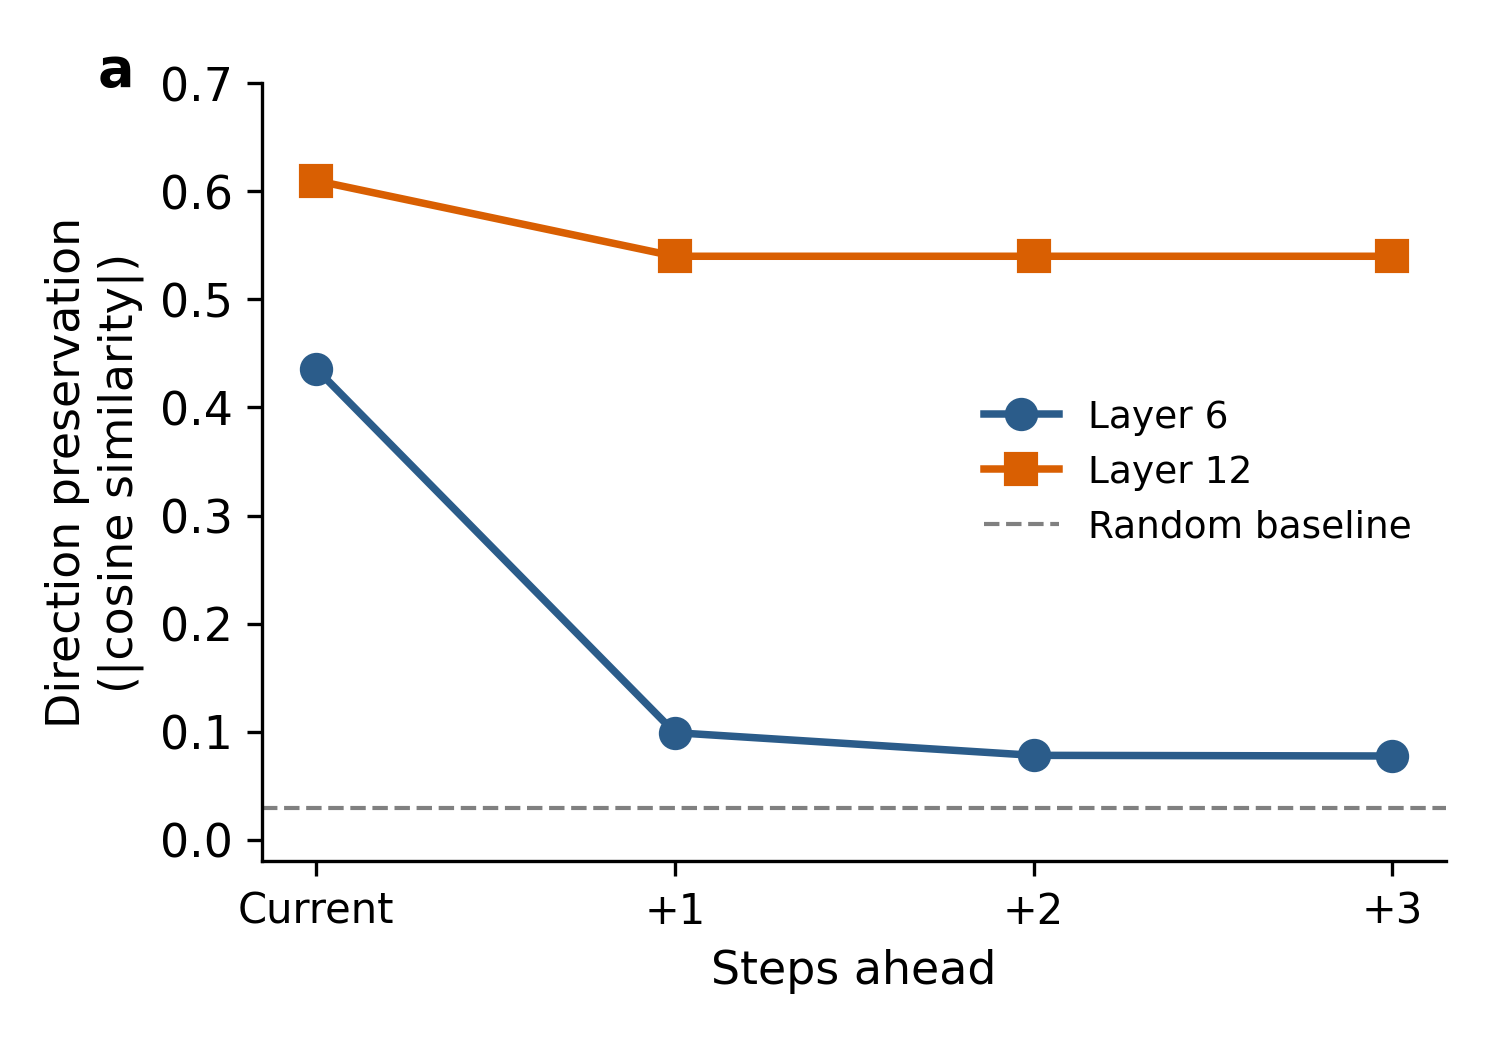
\includegraphics[width=0.8\textwidth]{fig4_direction.png}
\caption{Direction preservation decay by layer and steps ahead (Natural Stories). At layer 6, direction preservation drops from 0.44 at the current step to 0.10 at one step ahead, close to but above the random baseline, indicating that directional structure decays rapidly. At the final layer (layer 12), direction preservation remains elevated (0.54) across all steps ahead, indicating persistent directional structure. Dashed horizontal line indicates the random baseline for 768-dimensional vectors (0.029).}
\label{fig:direction}
\end{figure}

\new{\subsection{Neither Result Reduces to Constituent Structure}\label{sec:syntax}

The most serious alternative reading of everything above is syntactic. Words within a phrase are semantically and distributionally related, so their representations might move coherently for that reason alone; phrase boundaries might supply the turns; the trajectory measure might be a graded boundary detector; and its reading-time effect might be syntactic wrap-up. On that account there is no momentum and no trace of production---only grammar, viewed geometrically. We tested this in a preregistered analysis (criteria and outcome logic fixed in advance; the preregistration, including one operationalization deviation discovered and documented at analysis time, is in the repository).

Every word transition in the locked sample was classified against the corpus's constituency parses: brackets closed and opened at the transition, whether the two words share their immediately dominating constituent, and the depth of their lowest common ancestor (extraction validated at 100\% coverage and 99.9\% word-form agreement; brackets closed agrees with the sample's existing annotation at $r = .998$).

\paragraph{Geometry.} The syntactic account predicts directional coherence within phrases and collapse at boundaries, scaling with boundary depth. Neither happens. Direction preservation is flat across transition classes: .424 where the two words share a parent, .445, .428, and .451 as the lowest common ancestor recedes to three or more levels---deep boundary crossings are as directionally preserved as phrase-internal transitions, all roughly fifteen times the random baseline. Entered jointly, the full syntactic transition classification absorbs 3.1\% of the variance in alignment. The pre-specified criterion (mean alignment at deep transitions at least three times baseline) was passed at more than fifteen times.

\paragraph{Reading time.} The wrap-up account predicts the trajectory effect should live at constituent boundaries. It is strongest where no boundary exists. Restricting to transitions where no constituent closes and both words share a parent---positions at which nothing is wrapping---extrapolation error predicts reading time in 79.5\% of 161 participants ($\beta = +0.050$, Wilcoxon $p = 2.5 \times 10^{-18}$), passing the standing reliability criterion within the subset. At boundary transitions the effect is present but weaker (61.0\% of participants). This is the reverse gradient from the one syntactic wrap-up predicts. In the pooled model, the effect survives the full set of syntactic covariates.

Constituent structure, then, organizes the trajectory but does not explain it: syntax takes almost none of the directional coherence, and the behavioural effect is carried by phrase-internal positions where no syntactic event occurs. For completeness, the syntactic classification does absorb 8.7\% of the variance in the extrapolation-error measure itself, largely through brackets closed---the composite measure carries some boundary signal, but the reading-time effect does not depend on it.}

\new{\subsection{Beyond the Current Predictive Distribution}\label{sec:distsuff}

Everything so far shows the effect is beyond \emph{surprisal}. Surprisal is one number extracted from the current distribution, and a reader could be a pure current-distribution processor whose cost function uses more of that distribution than the probability of the observed word---its entropy, its confidence, its concentration. Such a reader would also show effects beyond surprisal. The preregistered analysis in this section asks whether the trajectory effect reduces to distribution shape, with criteria fixed in advance.

The descriptive fact that decides most of the question is visible before any model is fitted: extrapolation error is nearly orthogonal to the shape of the distribution. Its correlation with entropy is $.043$, with collision entropy $.062$, with top-token confidence $-.068$, and with top-ten mass $-.059$, while the four functionals correlate $.89$--$.98$ among themselves. The measure shares variance with surprisal ($r = .31$) but almost none with how peaked or uncertain the prediction is.

The model comparisons confirm what the correlations suggest. Adding all four functionals to the headline specification leaves the trajectory term untouched ($\Delta\text{AIC} = 78.4 \rightarrow 79.4$; $\beta = +0.0030 \rightarrow +0.0031$, $p = 1.8 \times 10^{-19}$), and the subject-level criterion is passed more strongly with the functionals in the model than without them: 74.7\% of participants positive against 67.8\% ($n = 174$; Wilcoxon $p = 1.3 \times 10^{-11}$).\footnote{The participant count differs marginally from the headline analysis (174 vs.\ 171) because merging the functionals changes row availability; comparisons within this analysis are like for like.} The matching analysis is the stringent version: within cells defined by joint quintiles of surprisal, entropy, and confidence (91 populated cells; median 4,853 usable observations per participant), where distribution shape is held coarsely fixed and only the trajectory relation varies, the effect is the strongest in the paper: 74.7\% of participants positive, Wilcoxon $p = 7.9 \times 10^{-14}$. Both preregistered criteria are passed.

The reading-time claim licensed by this section is accordingly stronger than ``beyond surprisal'': holding the current predictive distribution fixed---its value at the word, its entropy, its confidence, its concentration---words that depart from the fitted heading of the preceding states are read more slowly, in three quarters of participants. The functionals are those of GPT-2 Small, the paper's model throughout; that scope is stated rather than hidden.}

\subsection{\new{Model Scale and Architecture}}

The preceding analyses all use GPT-2 variants, which share the same architecture and learned absolute positional embeddings. To test whether the trajectory extrapolation effect depends on this specific positional encoding scheme, we replicated the Natural Stories analysis using Pythia models \citep{biderman2023}, which use Rotary Position Embeddings (RoPE), a fundamentally different approach that encodes position through rotation of the hidden-state vectors rather than through additive position embeddings. We tested Pythia-160M (comparable to GPT-2 Small; mid-layer 6 of 12) and Pythia-410M (comparable to GPT-2 Medium; mid-layer 12 of 24).

The core finding replicated across both architectures (Table~\ref{tab:crossarch}). \new{All three models were evaluated on identical rows and identical participants ($n = 812{,}730$, 178 participants). Trajectory extrapolation error predicted reading times beyond surprisal in both Pythia-160M ($\Delta\text{AIC} = 88.3$, $\beta = +0.0029$, $p = 2.0 \times 10^{-21}$) and Pythia-410M ($\Delta\text{AIC} = 400.2$, $\beta = +0.0065$, $p = 1.7 \times 10^{-89}$), against $78.4$ for GPT-2 Small on the same data.} Direction preservation showed the same rapid decay at the mid-layer, dropping from 0.42 to near-random levels within a single step for both Pythia models, confirming that the \new{rapid decay of directional structure} is not an artifact of GPT-2's coordinate system.

\begin{table}[!htbp]
\centering
\caption{Cross-Architecture Replication: Pythia (RoPE) vs.\ GPT-2 (Absolute Position Embeddings)}
\label{tab:crossarch}
\begin{tabular}{lccrcc}
\toprule
\textbf{Model} & \textbf{Pos.\ enc.} & \new{$\boldsymbol{\beta}$} & \textbf{$\Delta$AIC} & \textbf{Dir.\ pres.\ +0} & \textbf{Dir.\ pres.\ +1} \\
\midrule
GPT-2 Small (117M) & Absolute & \new{$+0.0030$} & \new{78.4} & 0.44 & 0.10 \\
Pythia-160M & RoPE & \new{$+0.0029$} & \new{88.3} & 0.42 & 0.13 \\
Pythia-410M & RoPE & \new{$+0.0065$} & \new{400.2} & 0.42 & 0.11 \\
\bottomrule
\end{tabular}

\smallskip
\footnotesize
\textit{Note.} $\Delta$AIC extrap / surprisal = improvement from adding trajectory extrapolation error to the model already containing surprisal and lexical controls. \new{All three models are evaluated on identical rows and identical participants ($n = 812{,}730$, 178 participants).} Direction preservation values are mean absolute cosine similarity between the fitted trajectory direction and the displacement vector at the current (+0) and next (+1) word positions.
\end{table}

\FloatBarrier

\new{\subsection{Production: Speakers Pause Before Trajectory Departures}\label{sec:production}

If the trajectory cost belongs to the processing system rather than to reading in particular, it should appear where language is generated, in the one currency production makes observable word by word: time. The analyses in this section were preregistered before any timing variable was related to the measure, with amendments (all documented in advance of each dependent variable's first contact with the predictor) recording two corpora whose word-level alignments turned out to tile---absorbing pauses into words---and therefore could not support the word-level test.

\paragraph{Buckeye.} In the full 40-talker corpus (255 sessions; 252,401 same-talker word transitions with only silence intervening; median 6,182 per talker), speakers pause longer before words with higher extrapolation error, with surprisal, all four distribution functionals, frequency, length, and position controlled and all variables demeaned within talker: mean talker-level coefficient $+0.037$, \textbf{67.5\% of talkers positive} (27 of 40), Wilcoxon $p = 2.9 \times 10^{-3}$; raw $r$ between the measure and log pause $= +0.056$. The standing criterion is passed. The discovery sequence is disclosed rather than collapsed: the effect was first found, under the same preregistration, in the 7 talkers whose data happened to be on hand (82.5\% of 40 sessions positive, $p = 8.7 \times 10^{-7}$, all seven talkers individually positive), and then replicated on the full corpus---that is, on 33 talkers the analysis had never touched---with the effect size essentially unchanged.

\paragraph{Switchboard.} In 2,435 telephone conversations (2.79 million transitions; 4,747 conversation sides with at least 200 each), the coefficient is again positive (mean $+0.032$, Wilcoxon $p = 5.0 \times 10^{-73}$) with 61.5\% of sides positive against the 65\% criterion: a partial replication, in precisely the pattern of the comprehension side, where Natural Stories (67.3\%) clears the bar and the larger conversational corpus (SAP, 61.1\%) shows the same-direction effect below it. In both modalities the effect is strongest in the cleaner, monologue-like corpus and attenuates, without reversing, in large-scale dialogue.

\paragraph{Boundary conditions.} The effect is word-grain. At intonation-unit launches in the Santa Barbara corpus (transcriber-coded hesitation marks; 38,696 launches) the criterion fails outright (49.2\% of conversations positive, $p = .78$), as it does for acoustic pauses at segment launches in AMI (47.1\% of meetings, $p = .71$). Where a speaker is launching a planning unit, whole-unit planning evidently dominates; the trajectory cost is visible in the flow of fluent speech, between a word and the next, which is the same grain at which the reading-time effect lives.}

\new{\subsection{The Structure in Text Is Absorbed by a Stronger Model's Distribution}\label{sec:content}

The results so far could invite a deflationary reading: perhaps the costs merely track statistical structure in the text that our particular model fails to capture. A preregistered content analysis addresses this directly, and its outcome is a null that does the paper considerable good. At each of 12,333 token positions in Natural Stories, we drew twenty samples from the model's own next-token distribution (temperature 1, no truncation), computed the trajectory deviation each candidate would produce, and took the mid-rank of the \emph{human} author's actual token among the twenty-one. If human text is exchangeable with draws from the distribution, these ranks are uniform with mean 0.5, regardless of any property of the deviation measure; a pseudo-target sampled from the same distribution and passed through the identical machinery serves as a negative control, and the analysis is interpretable only where that control is uniform. Under GPT-2 Small, the control passes (0.502) and the human token ranks reliably low (mean 0.485, all ten stories below 0.5, Wilcoxon $p = 1 \times 10^{-13}$): human continuations hug the model's trajectory more than the model's own samples do. The preregistered model ladder then decides what that means. Under GPT-2 XL---distribution and geometry both---the control passes (0.500) and the human effect vanishes entirely (0.501, CI [0.497, 0.506]). Whatever trajectory structure human text carries, a stronger model's conditional distribution already contains it.

Two conclusions follow, and the preregistration fixed both before the data were seen. First, the momentum-like structure of text is compiled statistics: it cannot support any claim about the producer's mechanism, and this paper makes none. Second, and decisive for everything above: a model whose distribution demonstrably absorbs the trajectory structure of the text (GPT-2 XL) is among the models whose surprisal the reading-time effect survives ($\Delta\text{AIC} = 95.7$ with XL surprisal controlled; $82.1$ with four surprisals jointly). If the processing costs merely reflected text statistics our controls missed, the model that captures those statistics should capture the costs. It does not. The trajectory dependency is in the processor, not the artifact.}

\FloatBarrier

\section{Discussion}

\subsection{Two Dimensions of Sequential Processing}

Surprisal-based accounts have been remarkably productive at predicting incremental processing costs, but they treat comprehension as a sequence of evaluations against a probability distribution and discard the temporal structure of how the interpretation has been evolving. The results presented here suggest that human readers are sensitive to that dynamical structure as well. Specifically, our results show that human language processing times are impacted by two dissociable properties of the incoming signal: the probability of each word given its context (surprisal) as well as the degree to which each word deviates from the short-horizon trajectory of the evolving representation (trajectory extrapolation error). Critically, the effect of trajectory extrapolation \new{is strongly supported in Natural Stories, partially replicates in a second self-paced reading corpus, and replicates across} diverse model architectures with fundamentally different positional encoding schemes (GPT-2's absolute embeddings and Pythia's Rotary Position Embeddings), confirming that it reflects genuine properties of the hidden-state dynamics rather than an artifact of any particular model's coordinate system.

Interestingly, surprisal and trajectory extrapolation error are \new{correlated but far from redundant ($r = .31$ in Natural Stories)}, making independent contributions to reading times. If both measures are derived from the same model processing the same text, why are they \new{not more closely aligned}? The answer is that they capture errors at different levels of the sequential process. Surprisal reflects the model's token-level prediction error: how unlikely was this specific word, given the full context? Trajectory extrapolation error reflects the representational reorientation cost: how much did the hidden state change direction, given where it had been heading? A word can be probable but trajectory-breaking (it was expected but redirects the interpretation), or improbable but trajectory-continuing (it was unlikely but keeps the representation moving in the same direction). The two dimensions are logically independent, and the \new{dissociation matrix shows that the distinction has consequences for reading time in both directions}.

\new{This does not mean that either measure resolves the standing difficulties for surprisal-based accounts. \citet{huang2024} report that language model surprisal does not explain the magnitude of syntactic disambiguation difficulty, with garden-path constructions showing the largest misalignment. Our item-level analysis of their materials reproduces this. Across 72 item $\times$ construction pairs, the ambiguous-minus-unambiguous difference in surprisal does not predict the corresponding difference in reading time once construction is controlled ($\beta = -0.035$, $p = .78$), and extrapolation error does no better ($\beta = -0.019$, $p = .89$). Moving from a model's output probabilities to the geometry of its internal states does not repair that misalignment.}

\new{One methodological point follows from the surprisal controls. Surprisal from larger, lower-perplexity language models is a \textit{weaker} predictor of human reading times \citep{oh2023b}, so substituting a larger model's surprisal makes for a less stringent control rather than a more stringent one: it absorbs less of the outcome variance, and any predictor entered alongside it will appear correspondingly stronger. We therefore evaluate extrapolation error against a control containing all four surprisal estimates entered together.}

The displacement control analysis in GPT-2 rules out the simplest alternative interpretation of the trajectory-extrapolation error finding: that it merely indexes the magnitude of representational change in the embedding space. \new{The two measures are strongly correlated ($r = .80$) and each predicts slower reading alone, but entered together only extrapolation error retains an effect; displacement contributes nothing. What predicts reading time is therefore not representational movement as such, but the component of that movement which departs from the established trajectory.} However, the core finding, that trajectory extrapolation error contributes to reading-time prediction beyond surprisal, is robust across architectures.

The trajectory effect in Natural Stories is small in absolute terms (the coefficient is modest and the variance explained is a fraction of what surprisal contributes), but it is theoretically diagnostic: it is consistent, independent of surprisal, and directionally specific in a way that the simplest alternatives do not predict. \new{It is not, however, more pronounced at the locus where the theory most clearly predicts it. At the disambiguating word of a garden-path sentence---the point at which an established interpretation is known to reverse---neither extrapolation error nor surprisal predicts which items produce larger reading-time costs. Whatever the measure indexes, it is not specifically the cost of the reversal that garden-path sentences epitomize, in which the ambiguous region builds an interpretive trajectory in one direction and the disambiguating word forces a sharp reversal of it. That intuition motivated the measure but is not supported by these data.} At minimum, the data point to two dissociable components operating at different timescales: one that evaluates each word against a probability distribution, and another that is sensitive to the short-horizon trajectory structure of the interpretation as it evolves across words.

These results support a more dynamical process of language comprehension in which the trajectory of the evolving interpretive state, not just its position at each moment, shapes how each new word is processed. However, our results specifically support local representational continuity over a few-word window, not long-range directional momentum: the direction-preservation analysis confirms that directional structure dies within a single word at the predictive layer, so the trajectory the measure captures is strictly short-horizon. This pattern suggests that a single mechanism, whether framed as prediction error, information-theoretic surprise, or Bayesian updating, does not fully account for the costs of incremental comprehension.

\subsection{Trajectory as a Functional Property of Language}

Why might language comprehension track this short-term trajectory structure? The answer, we suggest, lies in both how language is produced and processed. Human language production is a sequential, locally planned process: speakers and writers plan a few words ahead, execute that plan, and then re-plan \citep{levelt1989,ferreira2002}. \new{The production results give this suggestion empirical footing of the right kind. The content analysis (Section~\ref{sec:content}) shows that whatever coherence production leaves in text is absorbed into a strong model's conditional distribution---text alone cannot testify about the producer's mechanism. But production \emph{timing} can, and does: speakers hesitate before words that depart from the recent representational path, with the entire distribution controlled (Section~\ref{sec:production}). The sequential footprint of production shows up not as a residue in the signal but as a cost in the act, at the same few-word grain as the comprehension effect---and at that grain only, since unit launches, where deliberate planning dominates, show nothing.}

Language models learn this short-horizon trajectory structure because it is present in their training data: human-produced text carries the local continuity of human production planning. The model's hidden states come to reflect this structure as a statistical byproduct of learning to predict the next word well. But the model does not use trajectory for its own processing; the direction-preservation analysis shows that at the predictive layer, each word is effectively a fresh computation, with near-zero directional persistence from one step to the next. The model recomputes from full context at every position. The trajectory is in the representation, not in the processing strategy.

From the standpoint of comprehension, language processing also proceeds under strong recency constraints and limited working memory \citep{gibson1998,lewis2005}, so re-deriving the full interpretation from the entire preceding context at every word is not a tractable strategy. Some compressed summary of recent context is computationally necessary, and the local trajectory of the evolving interpretation is a natural candidate: it summarizes where the interpretation has been going over the last few words. A word that continues this local trajectory is cheap to integrate; a word that forces a deviation is expensive. The empirical question we addressed is whether human reading times are sensitive to this kind of local-continuity signal beyond what surprisal already captures.

Garden-path sentences are where the local continuity fails most dramatically. The local trajectory established by the ambiguous region points in the wrong direction, and the disambiguating word reveals that what looked like a coherent local trajectory was misleading. \new{That intuition motivated the measure, but the item-level analysis does not bear it out: neither extrapolation error nor surprisal predicts which garden-path items cost readers more, and coefficients standardised within participant are not comparable across corpora in any case.} But the phenomenon is not limited to garden paths. Any word that forces the representation off its recent trajectory incurs a cost, even in ordinary text, as demonstrated by the Natural Stories analysis.

This framing connects to lossy-context surprisal \citep{futrell2020}, which proposes that comprehenders work with a lossy representation of context rather than a perfect one. Trajectory extrapolation is a specific, extreme form of lossy context, perhaps the lossiest summary imaginable: a linear fit to three points in high-dimensional space. It also connects to the surprisal scaling paradox \citep{oh2023b}: as language models grow larger, their surprisal estimates reflect better full-context prediction, diverging from the recency-dominated processing that humans actually do. Our multi-model comparison offers a complementary perspective: while Oh and Schuler varied training data size, we varied model capacity within the same training data and found that the effect remains detectable across model sizes.

The kinds of words that populate the off-diagonal cells (reported in the Results) point to what the two measures are tracking. The low-surprisal / high-extrapolation cell is enriched for coordinators and complementizers (\new{``and'' at 3.9 times the corpus rate, ``as'' 3.6, ``had'' 3.5}), which are lexically routine connectives that open a new syntactic constituent whose hidden-state trajectory will be different in kind from the preceding one\new{, and for recurring story-specific proper nouns and content words (``bird'' 15.0, ``Elvis'' 14.9, ``manor'' 11.9), which are highly predictable within their narrative context but likewise begin a new constituent}. The high-surprisal / low-extrapolation cell is \new{depleted of closed-class items (31.6\% against a corpus baseline of 45.8\%) and enriched for} discourse pivots (\new{``now'', ``when'',} ``then''\new{)} that are lexically unexpected at that position but whose structural role the trajectory has already begun to accommodate. The pattern suggests that the trajectory dimension is sensitive to structural continuity (frame, theme, syntactic commitment), whereas surprisal indexes lexical identifiability over the full context. These appear to be different psycholinguistic constructs, and the dissociation observed in our regressions is consistent with that distinction.

\subsection{Prediction, Trajectory, and the Nature of Comprehension}

An intriguing question raised by these findings concerns the causal relationship between prediction and trajectory. In language models, trajectory structure is a byproduct of optimizing next-token prediction. The model learns to predict words, and trajectory emerges in the hidden states because human-produced text has momentum. Surprisal is the primary quantity; trajectory is secondary.

Whether the same priority holds in human comprehenders is an open question. One possibility is that prediction and trajectory sensitivity are genuinely independent components of processing, each contributing its own cost. Another, more speculative possibility is that the causal direction differs in humans: that comprehension is fundamentally a dynamical process in which the evolving representational state carries local trajectory continuity that is actively maintained and exploited, and that sensitivity to word-level probability arises partly as a consequence of this process rather than as a fully independent computation. Words that are improbable tend to be trajectory-breaking, which is why surprisal predicts processing costs; but some portion of what surprisal captures may reflect trajectory disruption rather than prediction error per se. The present data are consistent with both interpretations, and with intermediate accounts in which prediction and trajectory interact in ways that neither tradition has fully specified.

What the data do establish is that the two measures are dissociable \new{(correlated at $r = .31$ in Natural Stories, but with independent contributions to reading times)} and that this dissociation calls for explanation. A direct experimental test, constructing stimuli matched on surprisal but varying in trajectory disruption or vice versa, would provide sharper evidence about the relationship. The theoretical question of how prediction and trajectory relate in human processing remains open and experimentally tractable.

\new{\subsection{Mechanism in the Processor, Statistics in the Text}

The four results form a single dissociation. What people \emph{write} is statistically exhausted by a strong model's current predictive distribution: the content analysis could not tell human continuations from the model's own samples once the model was strong enough. What it \emph{costs} people to process language is not: reading time tracks the trajectory measure with the entire distribution controlled and matched, and so does the silent pause before a spoken word. The current predictive distribution is sufficient for the artifact and insufficient for the act, on both sides of the channel.

This is, we think, the correct home for the intuition that language ``has momentum.'' Any lawful trajectory structure in produced language is a statistical regularity, and statistical regularities are exactly what conditional models absorb---so the intuition could never have been vindicated in text, as our content analysis demonstrates by construction. It is vindicated, in a modest and specific form, in processing: the systems that produce and comprehend language pay a measurable cost when the next word departs from the recent representational path, a cost that no functional of the current distribution accounts for. The scope of the claim should be stated as carefully as its content. A sufficiently enriched instantaneous state can always render a system Markovian; what these data show is that the state variables standard theories treat as sufficient---the current predictive distribution in particular---are not sufficient for processing cost, while being fully sufficient for the produced signal. Whether the underlying neural computation maintains something like a representational heading is the natural next question, and it is answerable: the same measure can be regressed against time-resolved neural data, where the trajectory hypothesis predicts sensitivity to recent heading over and above the instantaneous predictive state.}

\subsection{Limitations and Future Directions}

\new{Several limitations should be noted. First, the effect is second-order relative to surprisal and to lexical frequency, and a substantial share of it is lexical: controlling word identity attenuates it substantially. It is a contribution to processing cost, not a rival account of it; the same is true of the production effect, which accounts for a small fraction of pause variance. Second, the garden-path materials comprise 24 items in each of three constructions, which is too few to support the item-level test those materials were included for; neither our measure nor surprisal predicts item-level variation in the size of the garden-path effect, and with three constructions the between-construction comparison rests on three points. Third, the comprehension evidence comes from self-paced reading, which delivers words serially and permits neither regressions nor parafoveal preview. Whether the effect extends to reading with free eye movements is not tested here, and claims about trajectory sensitivity in comprehension should be confined to serial presentation until it is. Fourth, the production result rests primarily on one corpus: Buckeye supplies the preregistered pass and its full-corpus replication, while Switchboard replicates direction and magnitude but falls below the sign-consistency criterion, and the register difference (interview monologue against telephone dialogue) is confounded with everything else that differs between the corpora. Fifth, the trajectory measure and the distribution functionals are computed from GPT-2 Small throughout; the surprisal controls span stronger models, but the geometry is one model's, and the distribution-sufficiency result (Section~\ref{sec:distsuff}) is stated for that model's functionals. Finally, the content analysis bounds its own interpretation: it shows the text carries no trajectory information beyond a strong model's distribution, not that the human production system lacks such information---timing, not content, is where that question is answerable, and where we answered it.}

The most promising future directions test the theoretical claims more directly. Constructing stimuli matched on surprisal but varying in trajectory disruption would provide the cleanest test of whether trajectory sensitivity is independent of word-level prediction\new{, and the tercile analysis reported above identifies where in the corpus such items are to be found}. Neural measures (EEG, MEG) could establish whether trajectory extrapolation error predicts brain responses independently of surprisal, moving the evidence from behavior to mechanism. \new{The restriction to serial presentation invites a specific design: presenting the same materials to the same readers under self-paced reading, serial visual presentation, and free eye movements would establish whether the effect depends on preview, on serial delivery, or on neither. Spoken presentation, which affords no preview either, would extend the same logic to the modality in which comprehension ordinarily occurs.}

A further implication concerns language generation. If local trajectory continuity contributes to processing ease, then human-produced and machine-produced text may differ in their trajectory statistics, and models or decoding strategies that preserve local trajectory coherence may yield text that is easier for humans to process. This remains speculative, but it offers a testable extension of the present framework.

\new{\section*{Data and code availability}

All analysis code, saved analysis outputs, and the locked measure samples are
available at \url{https://github.com/elanbarenholtz/garden-path-tee-curvature}.
The Natural Stories measure sample is identified by the fingerprint
\texttt{8a6087341e} and the garden-path measure sample by \texttt{e9fd2c547a};
both are asserted at the top of every script that uses them, so any analysis can
be traced to the exact rows it was computed on. The repository includes an
independent reimplementation of each measure pipeline
(\texttt{VERIFY\_sap.py}), written to different methods at every step, which
reproduces the reported values to $4.7 \times 10^{-16}$.

The reading-time corpora are third-party and are not redistributed here.
Natural Stories is available from \citet{futrell2018}. The Classic Garden Path
materials and reading times are part of the SAP Benchmark and are available from
\citet{huang2024}; the file is required to reproduce the garden-path row and
participant counts reported above. \new{The speech corpora are likewise
third-party: Buckeye \citep{pitt2007} by registration, Switchboard word
alignments from the public ISIP release \citep{godfrey1992}, the Santa Barbara
Corpus \citep{dubois2000} and AMI annotations \citep{carletta2007} from their
public distributions. The preregistrations for the distribution-sufficiency,
production-latency, and content analyses---including all amendments, each
committed before the relevant data were examined, and the complete outcome
logs---are in the repository under \texttt{gp\_confound\_check/}.}}

\bibliographystyle{apalike}
\bibliography{references}

\end{document}
